% Chapter Template

\chapter{Background} % Main chapter title

\label{Chapter2} % Change X to a consecutive number; for referencing this chapter elsewhere, use \ref{ChapterX}

%----------------------------------------------------------------------------------------
%	SECTION
%----------------------------------------------------------------------------------------

\section{Web Technology Stack}

%----------------------------------------------------------------------------------------
%	SECTION
%----------------------------------------------------------------------------------------

\section{HTML5 And Canvas API}

%----------------------------------------------------------------------------------------
%	SECTION
%----------------------------------------------------------------------------------------

\section{Mandelbrot Set}

The Mandelbrot set is a famous example of a fractal in mathematics. It is named after Beno\^{\i}t Mandelbrot, a Polish-French-American mathematician\footnote{ Its definition and name are due to Adrien Douady, in tribute to the mathematician Beno\^{\i}t Mandelbrot\cite{wiki:mandel}.}. The reason this thesis is using Mandelbrot set as the source of extreme resolution dataset is because Mandelbrot set can provide theoretically infitely high resolution datasets. In this section, we'll introduce briefly Mandelbrot set, its algorithms ideas for visualization.

\subsection{What Is Mandelbrot Set}

First we define a sequence

\[z_n, n = 0, 1, 2 ..\]

The initial value of $z$ is $z_0 = 0$. And then

\[z_1 = z_0^2 + c = c\]

Where $c$ is a constant in the complex plane.

The rest of $z_n$ is as follows:

\[z_{n+1} = z_n^2 + c\]

For different constant $c$, the absolute value of $z_n$ could remain bounded however large $n$ gets or be divergent.

The Mandelbrot set is the set of values of $c$ in the complex plane for which this sequence remains bounded.

\subsection{Important Properties of the Mandelbrot Set}

A property of Mandelbrot set is as follows:

A complex number $c$ belongs to the Mandelbrot set $M$, if and only if the absolute value of $z_n$ is not larger than $2$, for all $n = 0, 1, 2, ..$

\subsection{Simple Graphical Presentation}

The following figure \gmref{fig:mandelbrot} is a simple graphical representation of Mandelbrot set. A point $c$ in the complex plane is conventionally colored \emph{black} if it belongs to the Mandelbrot set $M$, and \emph{white} if not. 

\begin{figure}[th]
\centering
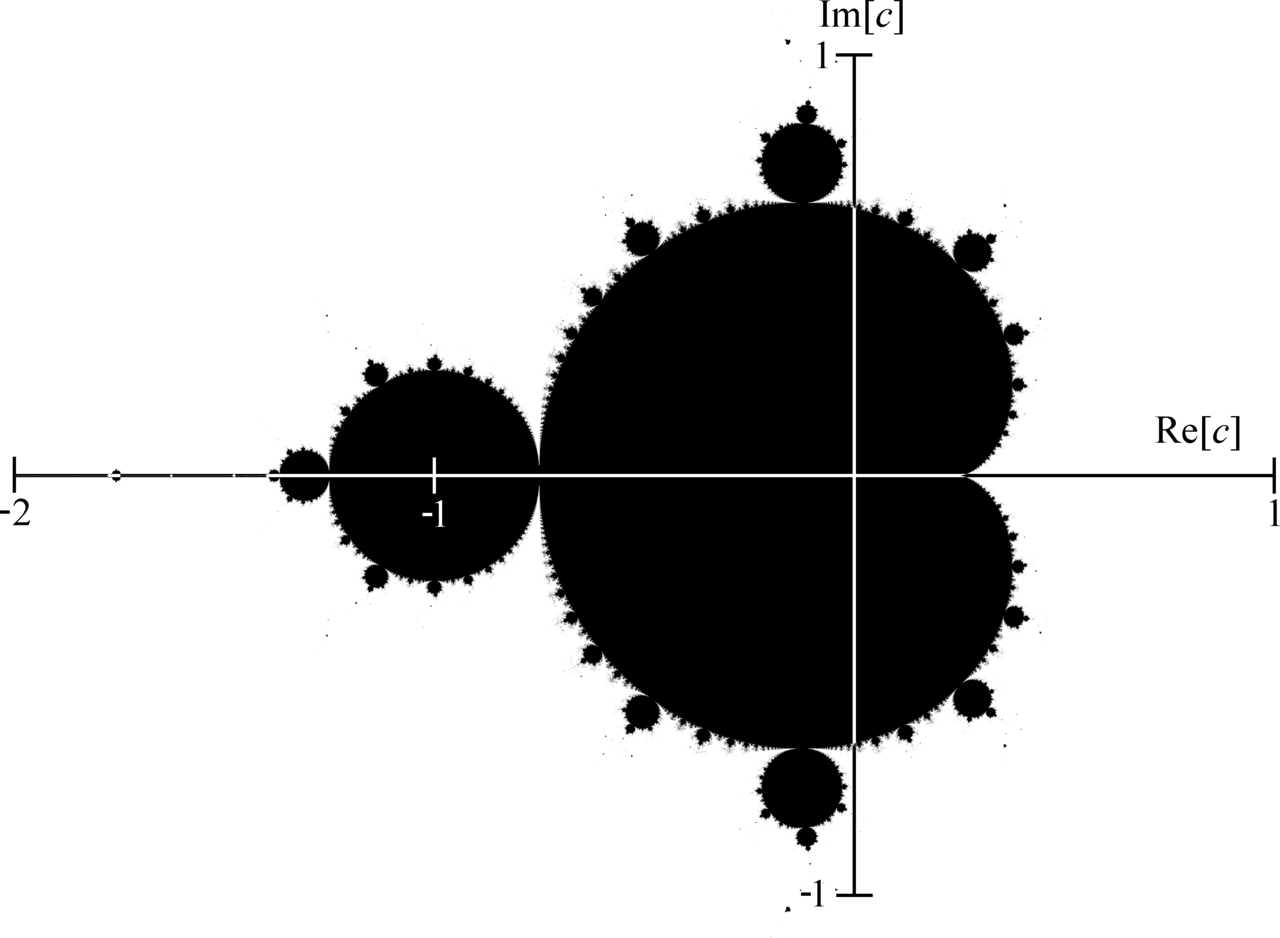
\includegraphics[width=\textwidth,keepaspectratio]{Figures/Chapter2/mandelbrot.png}
% 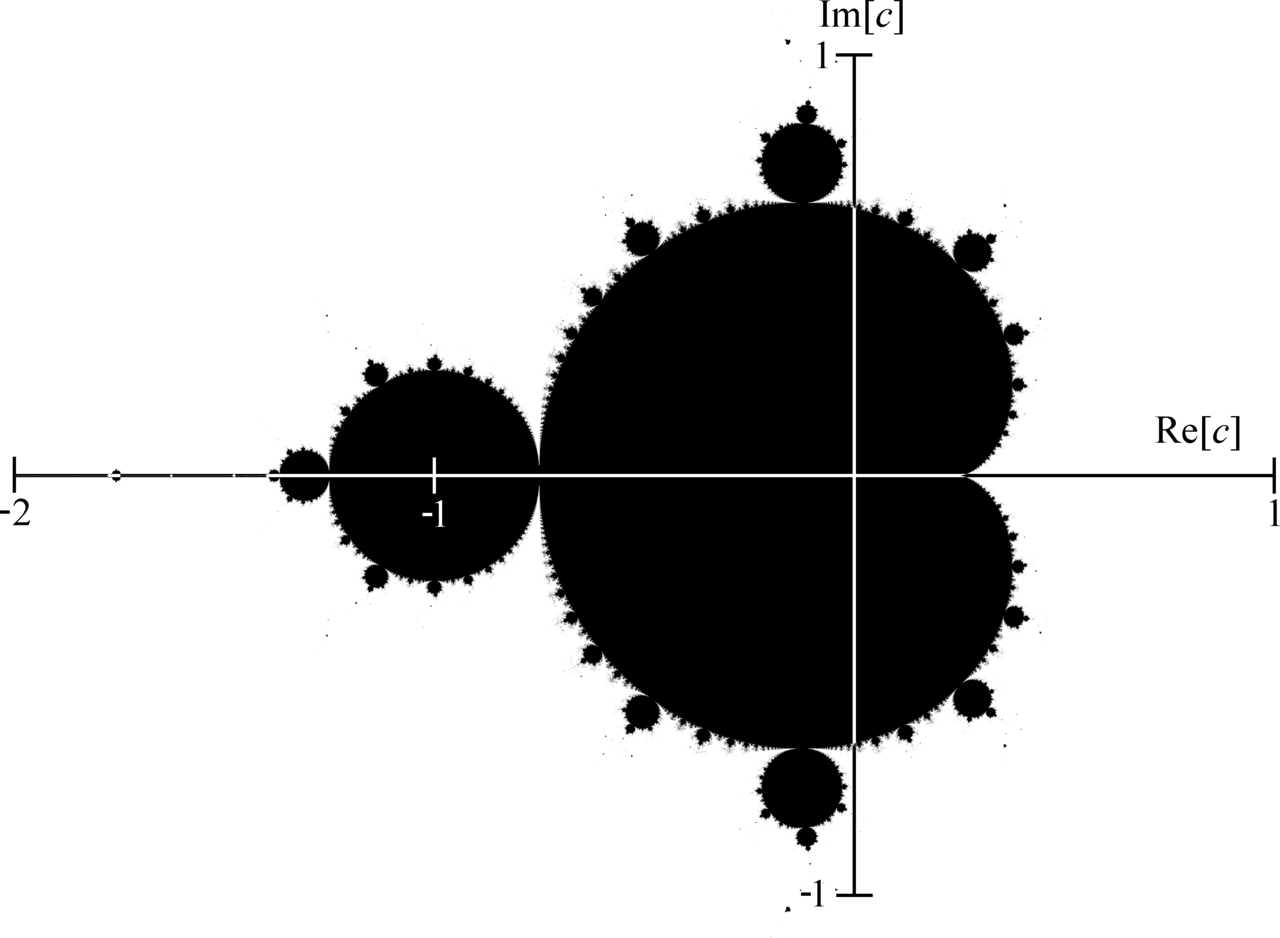
\includegraphics{Figures/Chapter2/mandelbrot.png}
\decoRule
\caption[Mandelbrot Set Graphical Presentation]{A simple graphical representation of Mandelbrot set.}
\label{fig:mandelbrot}
\end{figure}

\subsection{Algorithms For Visualization}\label{chap2:algorithmsforvisualization}

For all $c$ in complex plane:

~~~~For each $c$, we calculate sequence $z_n, n = 0, 1, .., max$:

~~~~~~~~$z_0 = 0$, (initial value),

~~~~~~~~$z_{n+1} = z_n^2 + c$

~~~~~~~~If the value of $z_{n+1}$ is larger than $2$, then:

~~~~~~~~~~~~\begin{minipage}[t]{0.9\textwidth} $c$ does not belong to $M$. In this case, we set the color of $c$ to \emph{white} and the calculation of sequence is stopped. \end{minipage}

~~~~~~~~If $n = max$, then:

~~~~~~~~~~~~$c$ belongs to $M$ and we set the color of $c$ to \emph{black}.

\subsection{Algorithms Idea For Graphical Representation with Grayscale}

In the above algorithm in \ref{chap2:algorithmsforvisualization} \nameref{chap2:algorithmsforvisualization}, $c$ is set to either \emph{black} or \emph{white}. If the iteration number $n$ is equal to the maximum iteration number $max$ and the value of $z_n$ still less than $2$, then $c$ has the color \emph{black}. If the iteration number $n$ is smaller than $max$ then at this moment the absolute value of $z_n$ becomes larger than $2$. In this case, we cannot set the color of $c$ to \emph{black}, because $c$ dose not belong to Mandelbrot set. However, we set a color with a portion of \emph{black}, to indicate how close $c$ is to be in \emph{black} area.

For all $c$ in complex plane:

~~~~For each $c$, we calculate sequence $z_n, n = 0, 1, .., max$:

~~~~~~~~$z_0 = 0$, (initial value),

~~~~~~~~$z_{n+1} = z_n^2 + c$

~~~~~~~~If the value of $z_{n+1}$ is larger than $2$, then:

\begingroup
    \leftskip=3em $c$ does not belong to $M$. In this case, we set the color of $c$ to \st{\emph{white}} \emph{grayscale\footnote{ In the current implementation, this color is set to be grayscaled red, rgb($grayscale\% \times 255$, 0, 0).} depending on the number of iteration} $n$ and the calculation of sequence is stopped.\par
\endgroup

~~~~~~~~If $n = max$, then:

~~~~~~~~~~~~$c$ belongs to $M$ and we set the color of $c$ to \emph{black}.